%%%%%%%%%%%%%%%%%%%%%%%%%%%%%%%%%%%%%%%%%%%%%%%%%%%%%%%%%%%%%%%%%%%%%%%%%%%%%%%%
%2345678901234567890123456789012345678901234567890123456789012345678901234567890
%        1         2         3         4         5         6         7         8

%\documentclass[letterpaper, 10 pt, conference]{ieeeconf}  % Comment this line out if you need a4paper

\documentclass[a4paper, 10pt, conference]{ieeeconf}      % Use this line for a4 paper



\IEEEoverridecommandlockouts                              % This command is only needed if 
                                                          % you want to use the \thanks command

\overrideIEEEmargins                                      % Needed to meet printer requirements.

% See the \addtolength command later in the file to balance the column lengths
% on the last page of the document

% The following packages can be found on http:\\www.ctan.org
%\usepackage{graphics} % for pdf, bitmapped graphics files
%\usepackage{epsfig} % for postscript graphics files
%\usepackage{mathptmx} % assumes new font selection scheme installed
%\usepackage{times} % assumes new font selection scheme installed
\usepackage{amsmath} % assumes amsmath package installed
%\usepackage{amssymb}  % assumes amsmath package installed
\usepackage{color}
\usepackage{graphicx}
\usepackage{caption}
\usepackage{subcaption}

\title{\LARGE \bf
Knowledge Acquisition for Mobile Autonomous Robots:\\
A Bayesian Approach  }


\author{Deebul Nair$^{1}$ ,  Tim Niemueller$^{2}$, Paul G. Pl\"{o}ger$^{1}$ and Gerhard Lakemeyer$^{2}$% <-this % stops a space
%\thanks{*This work was not supported by any organization}% <-this % stops a space
\thanks{$^{1}$Bonn-Rhein-Sieg University of Applied Sciences, Department of Computer Science,
Sankt Augustin, Germany,
        {\tt\small {<deebul.nair, paul.ploeger>}@inf.h-brs.de}}%
\thanks{$^{2}$Knowledge-based Systems Group,
RWTH Aachen University, Aachen, Germany 
        {\tt\small {<niemueller, gerhard>}@kbsg.rwth-aachen.de}}%
}


\begin{document}



\maketitle
\thispagestyle{empty}
\pagestyle{empty}


%%%%%%%%%%%%%%%%%%%%%%%%%%%%%%%%%%%%%%%%%%%%%%%%%%%%%%%%%%%%%%%%%%%%%%%%%%%%%%%%
\begin{abstract}

Knowledge representation and reasoning techniques have empowered autonomous robots to do more complex tasks with minimum supervision. A  challenge  that  has  long been neglected is how to acquire this knowledge. In this paper, we present novel approaches for autonomous knowledge acquisition in mobile robots. We show that our approaches is capable of:
(1) learning knowledge about the human presence in a home by a mobile autonomous robot (2) learning knowledge about user preferences in object placement. 

\end{abstract}


%%%%%%%%%%%%%%%%%%%%%%%%%%%%%%%%%%%%%%%%%%%%%%%%%%%%%%%%%%%%%%%%%%%%%%%%%%%%%%%%
\section{INTRODUCTION}
Autonomous robots to be accepted in human environments as companions should seek to adapt itself to its operating environment, especially to the humans within these environments.  In particular, domestic robots should learn about the environment, e.g. about the typical locations of particular types of objects, types of objects and also relation between objects. Additionally, domestic robots should learn about the preferences and routines of the individuals they are to serve and assist.
Robots should, for example, learn about the eating and drinking habits, the places at which they prefer to be seated, the  utensils  and  objects  they  prefer  to  use  for  particular  tasks, etc.  

To illustrate the relevance of the topics presented in this paper, we motivate our work using a typical task of a domestic service robot.   We assume that the robot is given the task of delivering Waldo's coffee cup to Waldo, which requires the robot to locate the coffee cup first and then to locate Waldo for delivering it to him. To begin the search for the coffee cup, it would help the robot to have some prior knowledge regarding Waldo's habits; in particular the typical locations where he keeps his cup. This enables the robot to funnel its search for the object from a large number of locations to the most probable ones. Once the coffee cup is located and grasped the robot needs to reason about where it can currently find Waldo for delivering it to him. This in turn, requires the robot to have knowledge about the likely locations of Waldo at that time.
This motivating example leads us to the two research topics in knowledge acquisition we address in this paper:
\begin{enumerate}
	\item How can a mobile robot acquire knowledge about where objects located in a home ?
	\item How can a mobile robot acquire knowledge about time based human presence in a home ?
\end{enumerate}

Current state of the art knowledge reasoning systems such as KnowRob \cite{c1} use publicly available knowledge bases like Cyc \cite{c2} and Open-Mind Indoor Common Sense (OMICS) database \cite{c3} for gaining base knowledge about environments.  Searching the web to find common places of object locations in mobile robots was demonstrated by \cite{c4}. Although these methods capture generic information of human environments they lack in capturing the knowledge about user preferences and habits. 

Our solution to this problem is acquiring new knowledge about the environment and human behaviours from the daily observations made by the robot. Mobile robots generate a lot of data, which is converted into information for use by the robot. The information is consumed immediately and discarded after use. In our example this information consist of the poses of objects and persons the robot generates while it interacts with them. In this work we collect this information and try learn from it, to generate new knowledge. In \cite{c5} user preferences in object locations and human presence were learned, but this approach needs a large amount of data. However the major challenge for learning using a mobile robot and no external sensors is the sparsity of information available. To overcome this challenge we use state-of-the-art  Bayesian  learning techniques such as graphical models, Dirichlet processes and probabilistic programming.    The  probabilistic  formulation of our approaches allows a robot to deal with sparsity in the observations and to easily add common sense prior knowledge.  We evaluate the above mentioned approaches on two datasets collected using autonomous mobile robots in domestic environments.  We evaluate our approach on two long term datasets, ARUBA \cite{c6} and KTH \cite{c5}. 


\begin{figure}[!tbp]
  \begin{subfigure}[b]{0.21\textwidth}
    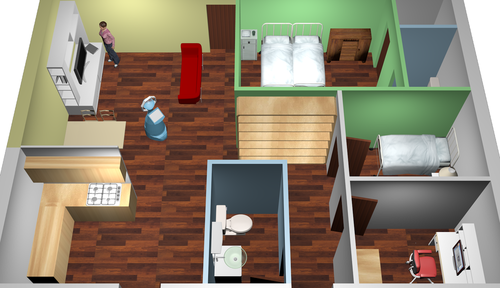
\includegraphics[width=\textwidth]{aruba-flat.png}
    \caption{human presence learning}
    \label{fig:f1}
  \end{subfigure}
  \hspace{1em}
  \begin{subfigure}[b]{0.21\textwidth}
    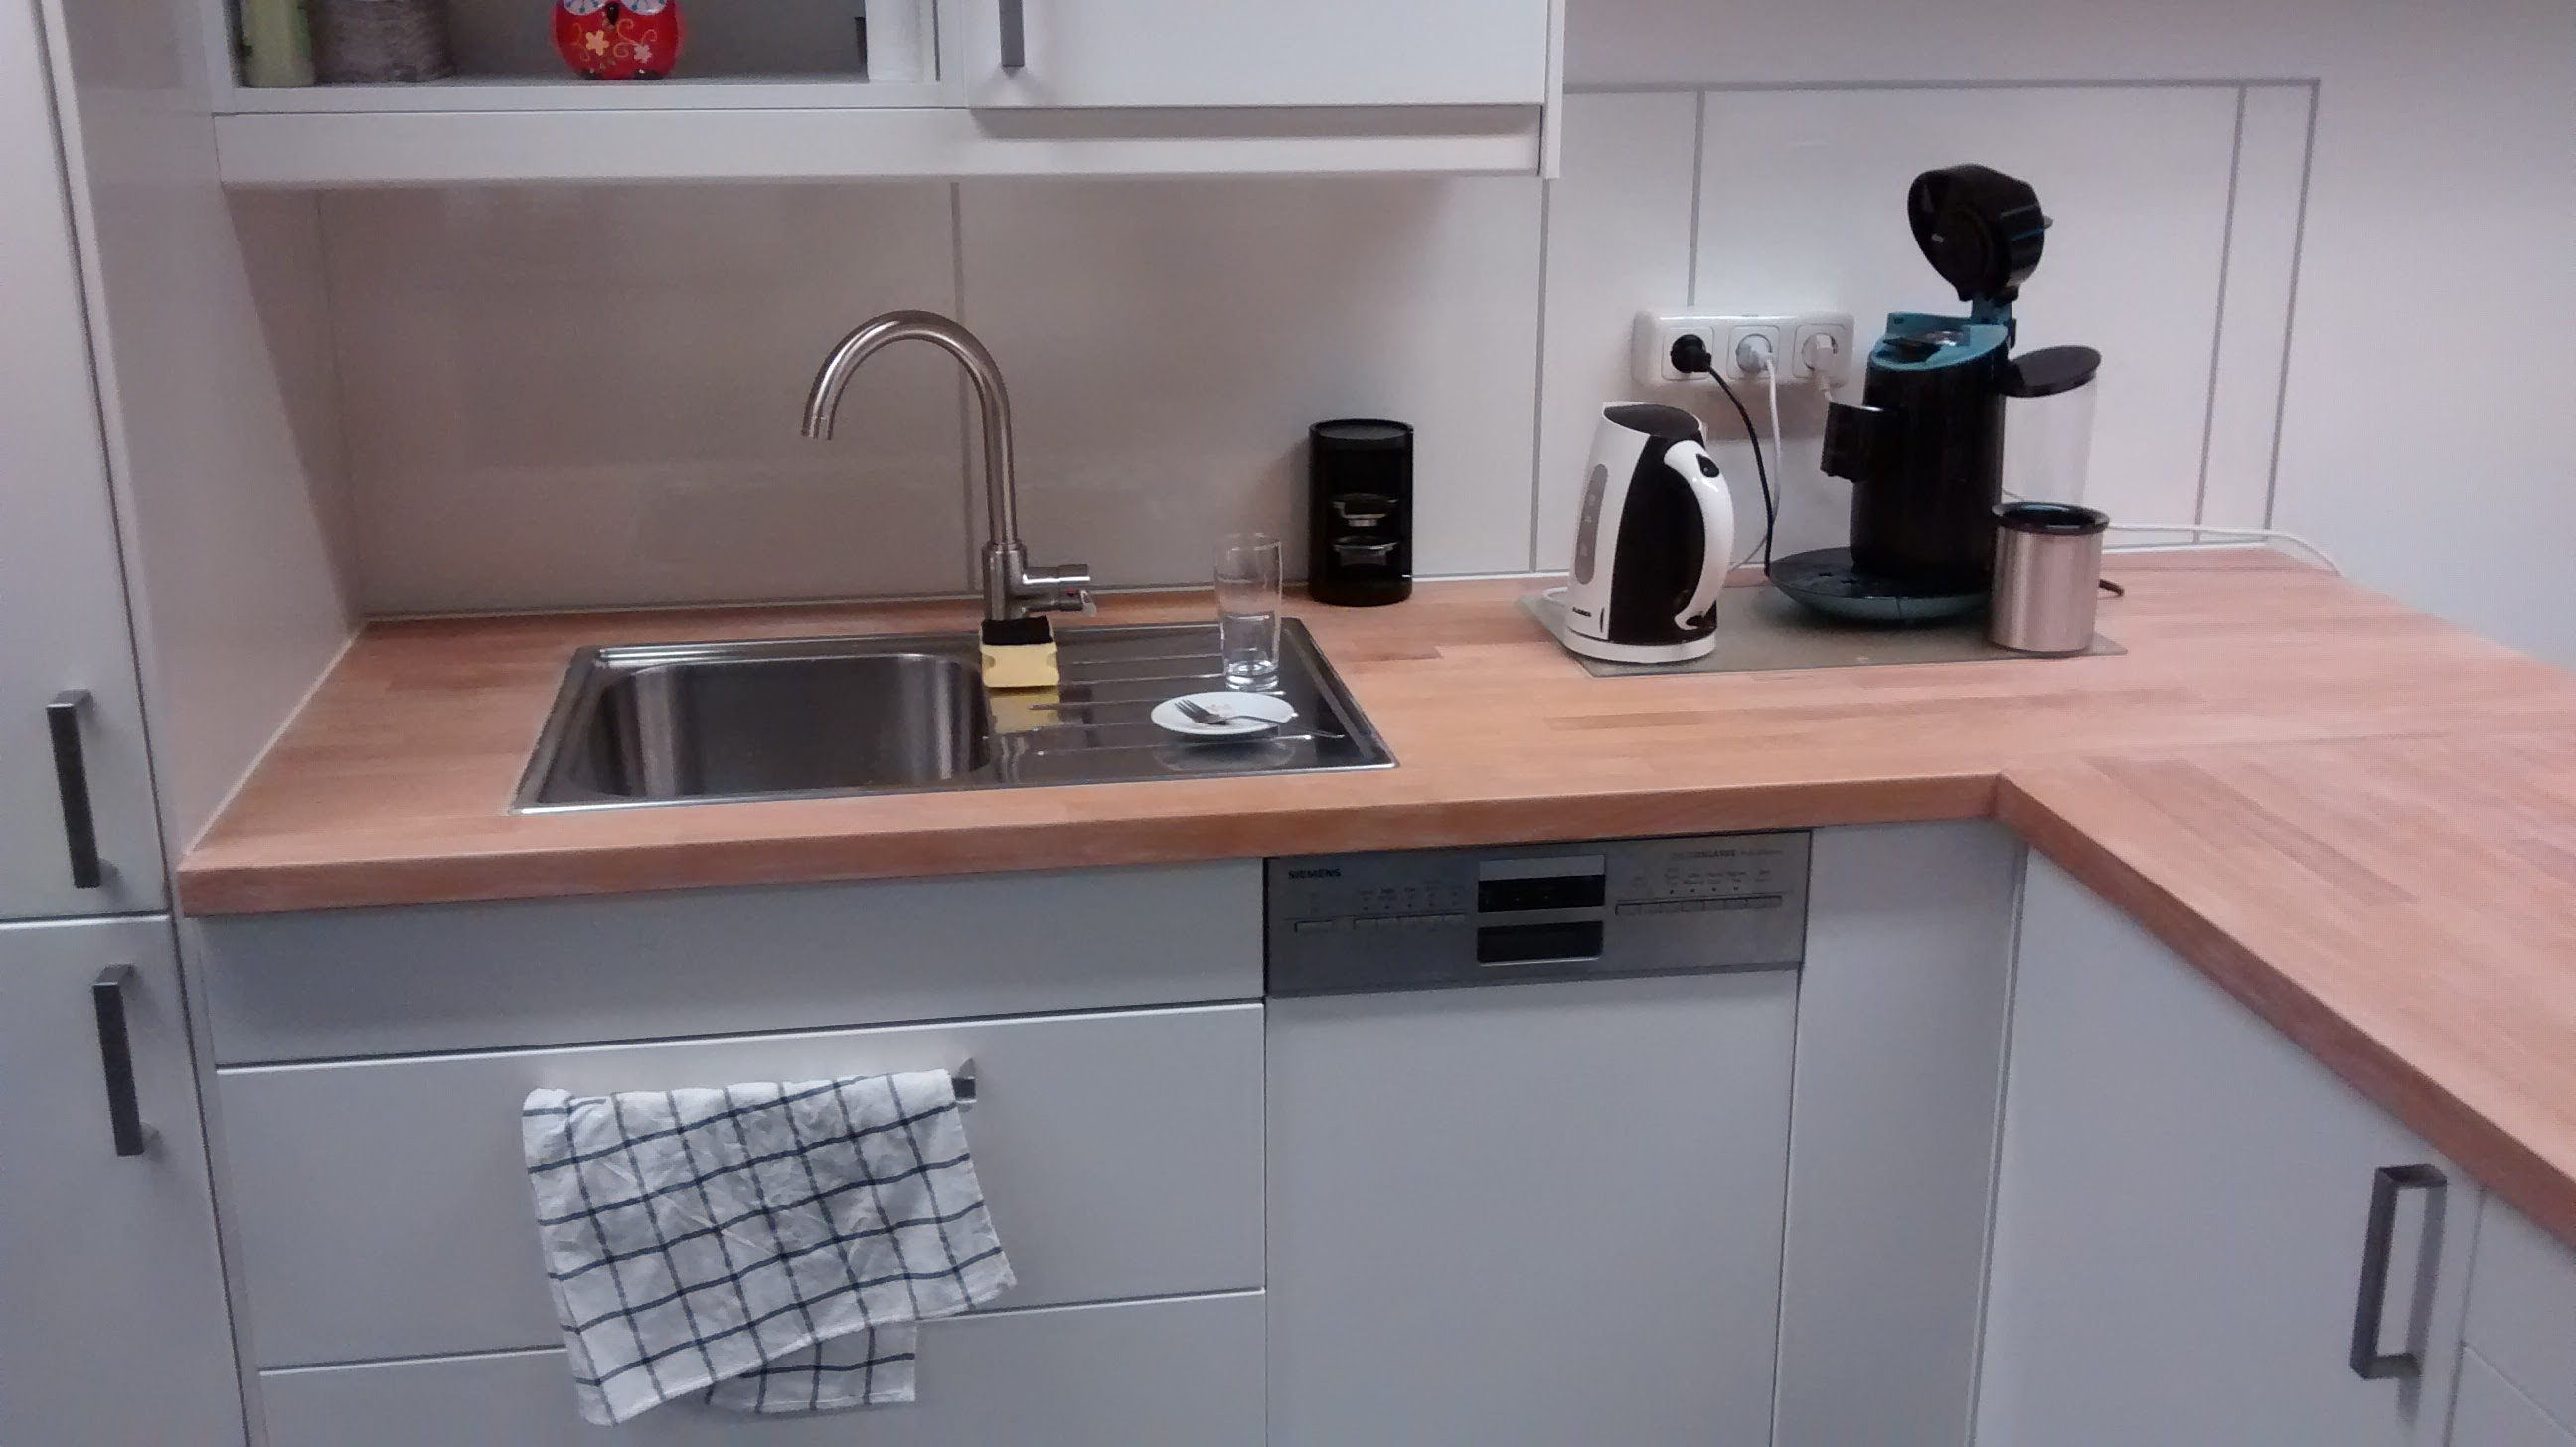
\includegraphics[width=\textwidth]{object_locations.jpg}
    \caption{object location learning}
    \label{fig:f2}
  \end{subfigure}
  \caption{Illustration of two setup of  knowledge acquisition. (a) Human presence learning from previous recorded Waldo’s locations. \cite{c5} (b) Object presence learning from previous observations}
\end{figure}
%%%%%%%%%%%%%%%%%%%%%%%%%%%%%%%%%%%%%%%%%%%%%%%%%%%%%%%%%%%%%%%%%%%%%%%%%%%%%%%%

\section{METHODS}

Bayesian models were developed to learn patterns in sparse data. Bayesian models can accommodate know beliefs into the model as prior, which enables learning from few data. It has been shown by research that humans exhibit periodic behaviour \cite{c7}. The behaviour is also replicated in how humans interact with the environment \cite{c8}. 
This information was included in the model as priors by making periodic temporal models.

\subsection{Human Presence : Dirichlet-Categorical Model}
Human can be present in only one of the location in the home at any instant of time. So we model this by using Categorical distribution. Dirichlet Distribution is the conjugate prior of Categorical distribution. The model is given below
\begin{gather*}
	\alpha = <1, 1, .... , 1 > \\
	\theta \sim Dirichlet(\alpha) \\
	y \sim Categorical(\theta)
\end{gather*}
where $\theta_i$ is the human presence distribution for time period $i$ and $y_{ij}$ is the data observed by the robot at location $j$ at time $i$ 
\subsection{Object Location : Beta-Bernoulli Model}
Object presence on a location is a boolean value, this is modelled using Bernoulli distribution. Beta Distribution is the conjugate prior of Bernoulli distribution. The model is given below
\begin{gather*}
	\alpha = 2 ; \beta = 2 \\
	\theta \sim Beta(\alpha, \beta) \\
	y = Bernoulli(\theta)
\end{gather*}
where $\theta_i$ is the confidence of presence of object in time period $i$ and $y_{ij}$ is the data observed by the robot at location $j$ at time $i$ 

\begin{figure}[!tbp]
  \center
  \begin{subfigure}[b]{0.2\textwidth}
    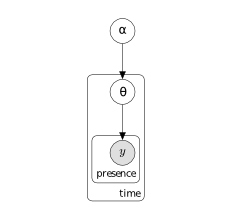
\includegraphics[width=\textwidth]{dirichlet-categorical.png}
    \caption{human presence model}
    \label{fig:f1}
  \end{subfigure}
    \hspace{3em}
  \begin{subfigure}[b]{0.2\textwidth}
    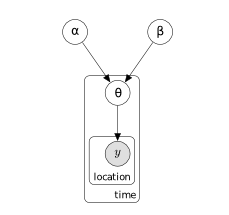
\includegraphics[width=\textwidth]{beta-bernoulli.png}
    \caption{object presence model}
    \label{fig:f2}
  \end{subfigure}
  \caption{Bayesian graphical models  (a) Human presence: Dirichlet-Catergorical Model (b) Object locations: Beta-Bernoulli model}
\end{figure}
%%%%%%%%%%%%%%%%%%%%%%%%%%%%%%%%%%%%%%%%%%%%%%%%%%%%%%%%%%%%%%%%%%%%%%%%%%%%%%%%

\section{EXPERIMENTS AND RESULTS}
To  evaluate  the  probabilistic  models,  we  performed  experiments on two  long-term  datasets.  Each  dataset  was  divided  into sparse training and testing sets. Human presence was learned on the  ‘Aruba’ dataset \cite{c6},  while user preference in object location was studied using the ‘KTH’ dataset \cite{c5}. 
\begin{figure}[!tbp]
  \begin{subfigure}[b]{0.243\textwidth}
    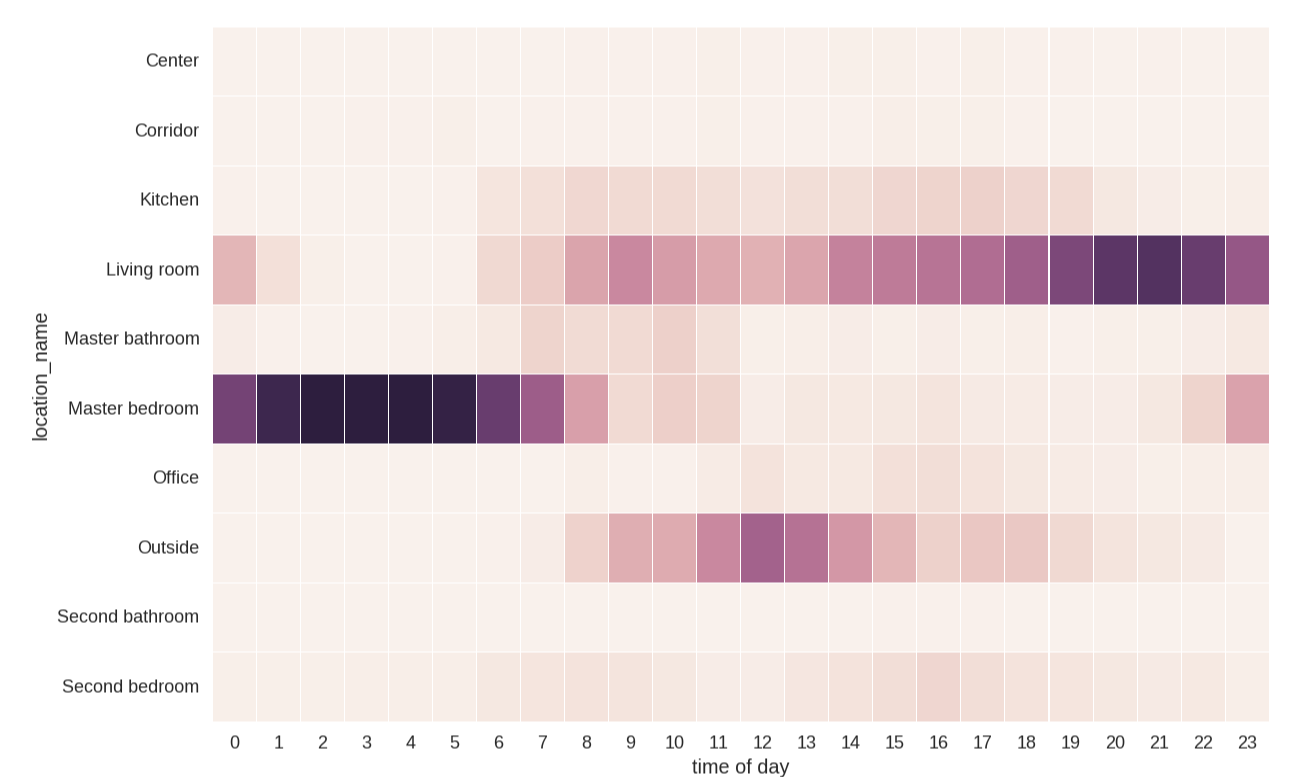
\includegraphics[width=\textwidth]{aruba.png}
    \caption{Ground truth heatmap}
    \label{fig:f1}
  \end{subfigure}
  \hspace{0.01em}
  \begin{subfigure}[b]{0.2\textwidth}
    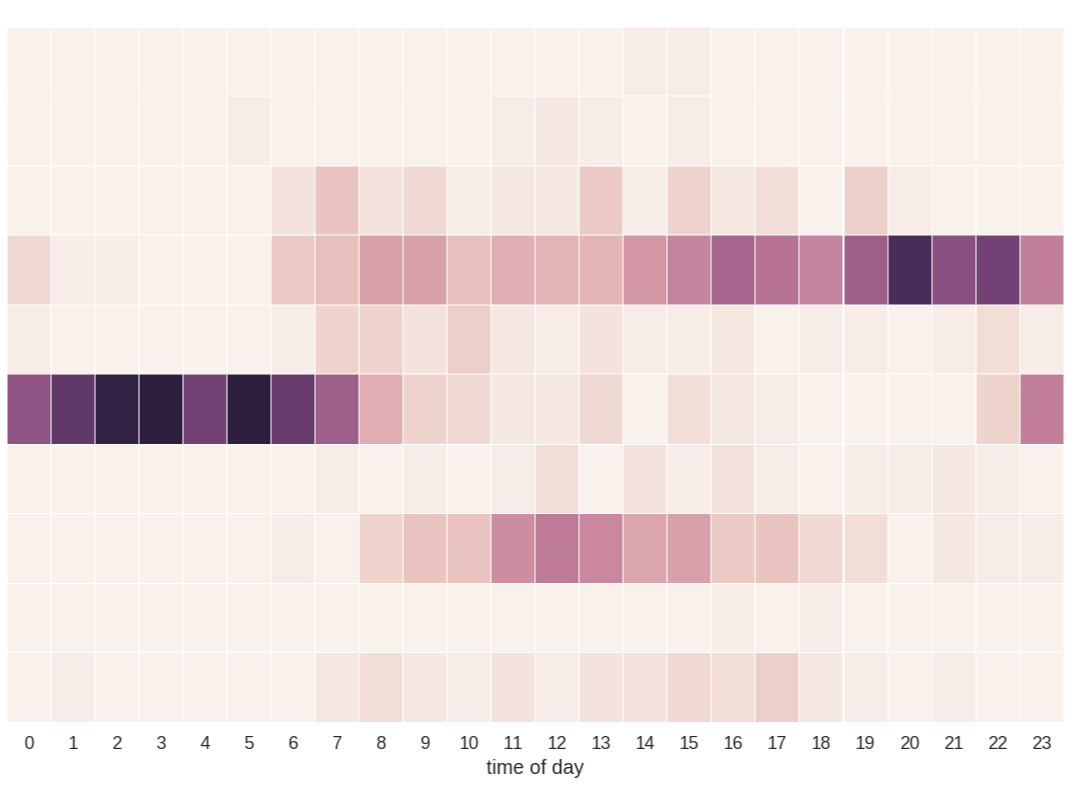
\includegraphics[width=\textwidth]{learned-aruba.png}
    \caption{Learned heatmap}
    \label{fig:f2}
  \end{subfigure}
  \caption{Evaluation of human presence learning. Heatmap of human presence on different locations based on time. (b) shows learned heatmap from a sparse dataset of the ground truth}
  \label{fig:f1_2}
\end{figure}
\subsection{ARUBA Dataset}
The  ‘Aruba’  dataset  consists of the location of a single person in a  seven room apartment every minute over a period of 16 weeks. In order to sparsify the data to resemble the data that would be collected by a real robot, we reduce the number of observations to 10 per day. In figure~\ref{fig:f1} we can see the pattern the user has over time over different locations. This can be compared with the learned model in figure~\ref{fig:f2}. The model has a prediction accuracy of 83.8\% .

\subsection{KTH Dataset}
The KTH dataset was collected by a SCITOS-G5 mobile robot in the Active Perception lab at KTH Stockholm, over  the  course  of  five  weeks.  During  this  time  the  robot conducted  between  two  and  six  autonomous  patrol  runs per  day,  visiting  three  specific waypoints  during  each  run and collecting information about the objects. A total of 36 objects were tracked over the period. As per the prediction accuracy results in Figure~\ref{fig:f3}, 21 objects had accuracy of above 80\% .
\begin{figure}[!tbp]
    \center
    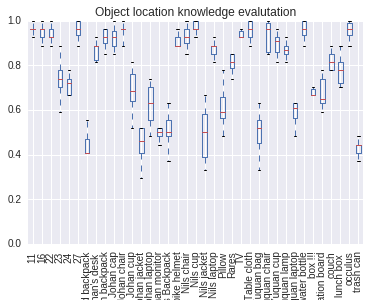
\includegraphics[width=0.4\textwidth]{learning_evaluation.png}
    \caption{Prediction accuracy of different objects}
    \label{fig:f3}
\end{figure}

%%%%%%%%%%%%%%%%%%%%%%%%%%%%%%%%%%%%%%%%%%%%%%%%%%%%%%%%%%%%%%%%%%%%%%%%%%%%%%%%

\section{CONCLUSIONS}

We think that the knowledge acquisition is growing need for knowledge and reasoning systems in mobile robots. In this work, we presented several innovative approaches of knowledge acquisition using a autonomous mobile robot with sparse information.   We  hope  that  our  work brings focus to field of autonomous knowledge acquisition.
\addtolength{\textheight}{-12cm}   % This command serves to balance the column lengths
                                  % on the last page of the document manually. It shortens
                                  % the textheight of the last page by a suitable amount.
                                  % This command does not take effect until the next page
                                  % so it should come on the page before the last. Make
                                  % sure that you do not shorten the textheight too much.

%%%%%%%%%%%%%%%%%%%%%%%%%%%%%%%%%%%%%%%%%%%%%%%%%%%%%%%%%%%%%%%%%%%%%%%%%%%%%%%%



%%%%%%%%%%%%%%%%%%%%%%%%%%%%%%%%%%%%%%%%%%%%%%%%%%%%%%%%%%%%%%%%%%%%%%%%%%%%%%%%
\section*{APPENDIX}
\subsection*{Probabilistic Programming: }
Probabilistic Programming gives us a framework in which we can create any model, based on our assumptions of the process. The model is basically expressing the assumptions in a mathematical form. The assumptions are the number of variables in the model, the relation between these variables, changes in which variables affects which other variables. This model is then used to generate a problem specific algorithm which can be used to solve the machine learning problem in hand. 
In this paper two probabilistic programming libraries were explored to create the models and infer, PyMC3\cite{c9} and BayesPy\cite{c10}

PyMC3 is python module for Bayesian programming. It provides intuitive model specification syntax for designing the models. The inference is primarily focussed on advanced Markov chain Monto Carlo fitting algorithms.

BayesPy provides tools to do probabilistic programming. In BayesPy users construct their models, observes data and then runs inference. The inference engine present in BayesPy is variational Bayesian inference.


%%%%%%%%%%%%%%%%%%%%%%%%%%%%%%%%%%%%%%%%%%%%%%%%%%%%%%%%%%%%%%%%%%%%%%%%%%%%%%%%

\section*{ACKNOWLEDGMENT}
The authors wish to thank Dr. Jaakko Luttinen, Alto University for his technical assistance throughout the project.

%%%%%%%%%%%%%%%%%%%%%%%%%%%%%%%%%%%%%%%%%%%%%%%%%%%%%%%%%%%%%%%%%%%%%%%%%%%%%%%%



\begin{thebibliography}{99}

\bibitem{c1} Moritz Tenorth and Michael Beetz. KnowRob -- A Knowledge Processing Infrastructure for Cognition-enabled Robots. In International Journal of Robotics Research (IJRR), volume 32, 2013. 
\bibitem{c2}  C.  Matuszek,  J.  Cabral,  M.  Witbrock,  and  J.  DeOliveira.   An introduction  to  the  syntax  and  content  of  Cyc. Proceedings  of the  2006  AAAI  Spring  Symposium  on  Formalizing  and  Compiling  Background  Knowledge  and  Its  Applications  to  Knowledge Representation and Question Answering, pages 44-49, 2006. 
\bibitem{c3}  Rakesh Gupta and Mykel J. Kochenderfer.  Common sense data acquisition  for  indoor  mobile  robots.In Nineteenth  National Conference  on  Articial  Intelligence  (AAAI-04,  pages  605-610),2004.

\bibitem{c4} Samadi Mehdi, Thomas Kollar, and Manuela M. Veloso. Using the Web to Interactively Learn to Find Objects. In AAAI, 2012. 

\bibitem{c5} Krajnik, Tomas, Miroslav Kulich, Lenka Mudrova, Rares Ambrus, and Tom Duckett. Where’s Waldo at Time T? Using Spatio-Temporal Models for Mobile Robot Search. In Robotics and Automation (ICRA), 2015 IEEE International Conference on, 2140–2146.
\bibitem{c6} D.  J.  Cook,  Learning  setting-generalized  activity  models  for  smart spaces, IEEE Intelligent Systems, vol. 2010, no. 99, p. 1, 2010.

\bibitem{c7} J. McInerney, A. Rogers, and N. R. Jennings, Learning periodic human behaviour models from sparse data for crowdsourcing aid delivery in developing countries, arXiv preprint arXiv:1309.6846, 2013.

\bibitem{c8} E. Cha, J. Forlizzi, and S. S. Srinivasa Robots in the Home: Qualitative and Quantitative Insights into Kitchen Organization, 2015, pp. 319–326.

\bibitem{c9} Salvatier, J., Wiecki, T., and Fonnesbeck, C. (2015). Probabilistic Programming in Python using PyMC. arXiv preprint arXiv:1507.08050

\bibitem{c10} J Luttinen. BayesPy: variational Bayesian inference in Python, Journal of Machine Learning Research, 2016







\end{thebibliography}




\end{document}
